\begin{frame}
\frametitle{Shopping list: hardware for this course}
  \begin{columns}
    \column{0.75\textwidth}
    \footnotesize
    \begin{itemize}
      \item STMicroelectronics STM32MP157D-DK1 Discovery kit -
        Available from Mouser (65 EUR + VAT)
      \item USB-C cable for the power supply
      \item USB-A to micro B cable for the serial console
      \item RJ45 cable for networking
      \item Nintendo Nunchuk with UEXT connector
            \footnote{\tiny \url{https://www.olimex.com/Products/Modules/Sensors/MOD-WII/MOD-Wii-UEXT-NUNCHUCK/}}
      \item Breadboard jumper wires - Male ends (to connect the Nunchuk)
            \footnote{\tiny \url{https://www.olimex.com/Products/Breadboarding/JUMPER-WIRES/JW-110x10/}}

      \item A standard USB audio headset.
      \item A micro SD card with at least 1 GB of capacity
    \end{itemize}
    \column{0.25\textwidth}
    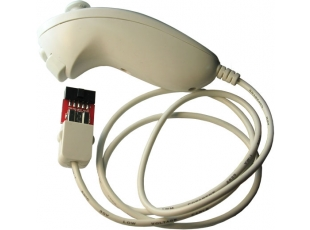
\includegraphics[height=0.25\textheight]{common/nunchuk.jpg} \\
    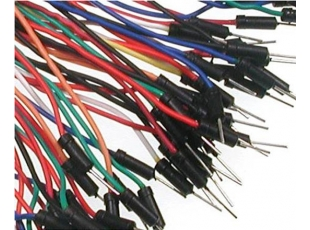
\includegraphics[height=0.15\textheight]{common/jumper-wires.jpg} \\
    %% Source: https://commons.wikimedia.org/wiki/Category:USB_Audio#/media/File:Andrea_Electronics_PureAudio_Speech_Development_Kit_(26603532598).png
    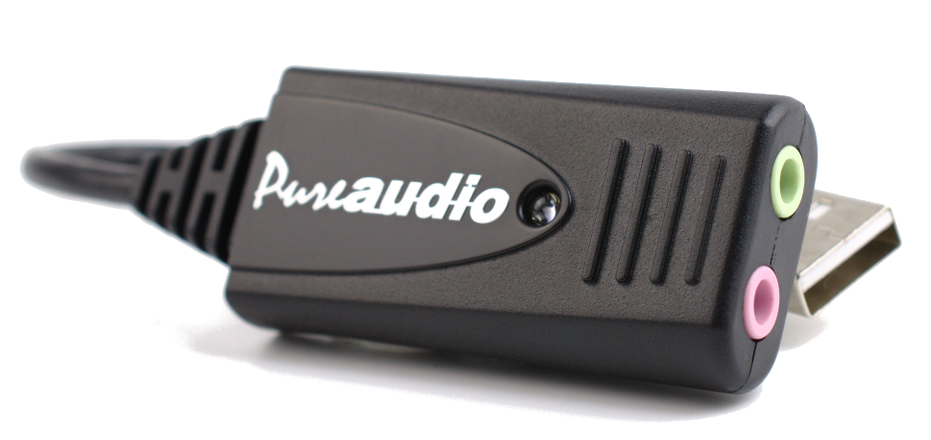
\includegraphics[height=0.15\textheight]{common/usb-audio.png} \\
    %% Source: https://commons.wikimedia.org/wiki/File:SD_card_icon.svg
    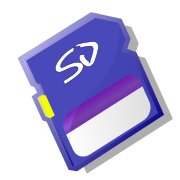
\includegraphics[height=0.15\textheight]{common/sd-card.pdf}
  \end{columns}
\end{frame}
